\documentclass[twocolumn]{aastex631}
% NOTE: Your template uses \documentclass[twocolumn]{aastex631} and
% \bibliographystyle{aasjournal}. This TeX installation ships the current
% AAS release (aastex701 + aasjournalv7) instead, which is structurally
% identical. To compile against aastex631, change the two lines back.

\newcommand{\vdag}{(v)^\dagger}
\newcommand\aastex{AAS\TeX}
\newcommand\latex{La\TeX}

\usepackage{gensymb}
\usepackage{amsmath}
\usepackage{array}
\usepackage{tabularx}
\usepackage{xfrac}
\usepackage{threeparttable}
\usepackage{xcolor}

% ---------------------------------------------------------------------------
% Figure placeholder: renders a labeled gray box in place of a real figure.
% Replace \figplaceholder{figN} with \includegraphics[width=\linewidth]{figN}
% once the real figure files are available.
% ---------------------------------------------------------------------------
\newcommand{\figplaceholder}[1]{%
  \setlength{\fboxsep}{0pt}%
  \fcolorbox{gray}{gray!12}{%
    \begin{minipage}[c][0.60\linewidth][c]{0.985\linewidth}%
      \centering
      {\Huge\bfseries #1}\\[6pt]
      {\large\color{gray} placeholder figure}
    \end{minipage}}%
}
% Shorthand for commonly repeated symbols
\newcommand{\rperp}{r_{\perp}}
\newcommand{\rparl}{r_{\parallel}}
% \newcommand{\rhoO}{\rho_0}
% \newcommand{\rO}{\r_0}
% \newcommand{RT}{R_\mathrm{T}}
% \newcommand{tdep}{t_\mathrm{dep}}
% \newcommand{xhat}{\hat{x}}
% \newcommand{yhat}{\hat{y}}
% \newcommand{zhat}{\hat{z}}
% \newcommand{\cosi}{\cos i}
% \newcommand{\Msun}{M_\odot}
% \newcommand{cm3}{\mathrm{cm^{-3}}}
% \newcommand{deg}{\degee}


\begin{document}

\title{The Global Structure of Molecular Clouds. II. Volume-Density Distributions}

\author[0009-0004-7985-6342]{Thummim Mekuria}
\email{tmekuria@ucsc.edu}
\affiliation{University of California, Santa Cruz \\
1156 High Street, Santa Cruz, CA 95064, USA}


\author[0000-0002-6001-598X]{Nia Imara}
\email{nimara@ucsc.edu}
\affiliation{University of California, Santa Cruz \\
1156 High Street, Santa Cruz, CA 95064, USA}

\author{John C. Forbes}
\email{john.forbes@canterbury.ac.nz} 
\affiliation{School of Physical and Chemical Sciences--Te Kura Mat\=u \\
University of Canterbury, Christchurch 8140, New Zealand}
\affiliation{Center for Computational Astrophysics \\
162 5th Avenue, New York, NY 10010, USA}

\begin{abstract}
We test a cylindrical model for the large-scale, global 3D structure of molecular clouds with observations of dust-extinction in the Solar Neighborhood. \textcolor{cyan}{we fit a linear spine to each cloud and measure how the length and orientation of the spines change for different clound boundaries. the volume density $\rho(r)$ decreases with perpendicular distance $r_\perp$ from the spine, with $\alpha \in ()$. the central density $\rho_0$ is negatively correlated with the turnover radius $r_0$, and (another relationship involving \rhoO} volume density distribution of gas and its relationship to star formation. We \textcolor{cyan}{fit the profiles over a range of distance bins and} We find that there is a \textcolor{cyan}{x type of relationship between the central volume density of a cloud $\rho_0$ and the turnover radius $r_0$. additionally, [this] is the relationship with mass. mass is also correlated with depletion time as [relationship], which is <robust to / depends on> some other factor that mass is usually connected to in the models. what are the implications of these results in terms of further developing the physical model. what are the implications of this wrt the field / ie where is it situated.}
\end{abstract}

\keywords{Molecular clouds (1072) --- Interstellar medium (847) --- Star formation (1569) ---
Interstellar dust extinction (837) --- Interstellar dust (836) ---
Interstellar filaments (842)}

%%%%%%%%%%%%%%%%%%%%%%%%%%%%%%%%% INTRODUCTION %%%%%%%%%%%%%%%%%%%%%%%%%%%%%%%%%%
\section{Introduction}\label{sec:intro}
\textcolor{cyan}{more ab morphology: works since this one that are about three-dimensional structure, big picture theory: enrique's work on filamentary flow, and lla10 on star formation, observations: dust-extinction derived maps}

\textcolor{cyan}{the structure of molecular clouds affects the efficiency of star formation, which makes it a key value in developing a complete picture of galaxy evolution. \citet{Larson1981} was the first to characterize the global structure of molecular clouds, through a systematic [survey of molecular lines in] of molecular clouds in [regions]. he found that $m \propto r^2$, implying molecular clouds have constant surface density. x many years later, phillips compiled a catalog of () star-forming regions and found that (). has there been large-scale (eg rosolowsky?) measuring and fitting the m vs r of molecular clouds either in the milky way or m33}

\textcolor{cyan}{dust is well mixed with the gas with a dtg ratio of (). however, the claim to constant surface density is (less valid - but first check if co derived measurements had already thrown questions on the third law) when measuring the m and r of molecular clouds from dust extinction (cite people who have looked at dust for m vs r, incl lewis). \citet{Lombardi2010} found that molecular clouds have column density values that span more than two orders of magnitude,}
\textcolor{cyan}{the larson scaling laws might also arise from the properties of observations (citations of people who have looked at this). \citet{BallesterosParedes2012} demonstrated defining the boundaries of clouds with extinctions that correspond to column densities near the peak of the pdf can artificially produce clouds with constant surface density. any other derivations of observational methods vs real physical structure}

\textcolor{cyan}{observations of clouds as filamentary structures at
range of spatial scales, from cores (citations) to spinal arm level (citaton)
($\sim$10--100~pc) \citep[e.g.,][]{Andre2010, Molinari2010, Li2013, Zucker2018,
Zhang2019, Schisano2020, Wang2020} there was that one paper about the bones of the milky way.  \citet{Neralwar2022} identified a population of more than 10,000 molecular clouds and found that 57\% are elongated.filfinder. also how do you get a cylinder from collapse happening along the shortest axis. the variations in surface density in molecular clouds have been shown to be realated to the evolutionary stage and star formation efficiency of clouds.}

\textcolor{cyan}{imara and forbes develop that the cylindrical model of molecular clouds parameterized by the central density, turnover radius and fall-off slope. they show that - what are the relationships between r0 and sfr / depletion time. imara forbes fit to surface density extinction maps. this means that the line of sight distribution of the gas is (). }

\textcolor{cyan}{in this work, we apply the imara forbes cylindrical model to three-dimensional reconstructions of molecular clouds in the solar neighborhood. what else do we do }

\textcolor{cyan}{we find that : key results 1 2 3.}

%%%%%%%%%%%%%%%%%%%%%%%%%%%%%%%%%%% THE MODEL %%%%%%%%%%%%%%%%%%%%%%%%%%%%%%%%%%%
\section{Background}\label{sec:model}
\subsection{the model}

\textcolor{red}{\textcolor{cyan}{talk about Zucker paper where they identify spines} Surface density maps of Galactic molecular clouds show that they often have elongated shapes, with much of their high-column-density gas concentrated along a central axis. For such clouds, one might reasonably assume---as we do here---that this elongated appearance is because their 3D morphology is cylindrical. Some computer simulations show that structures appearing to be filamentary/cylindrical are sometimes more flattened, sheet-like structures viewed in projection \citep[e.g.,][]{Imara2021}. Recent observational work by \citet{Tritsis2022} and \citet{Rezaei2023} to infer the volume density structure of molecular clouds using dust maps supports this view. In this study, we model molecular clouds as cylinders and choose a sample of clouds that appear to approximate this morphology. We will consider other geometries in future work.}

\textcolor{red}{One of our goals is to tease out information about the volume density
distribution of gas that has been projected onto the plane of the sky in surface density maps. Rather than trying to capture all of the intricate substructure known to comprise molecular clouds---e.g., filaments, clumps, and cores---our goal is to characterize their large-scale, global structure.}


\begin{figure*}[ht!]
\centering
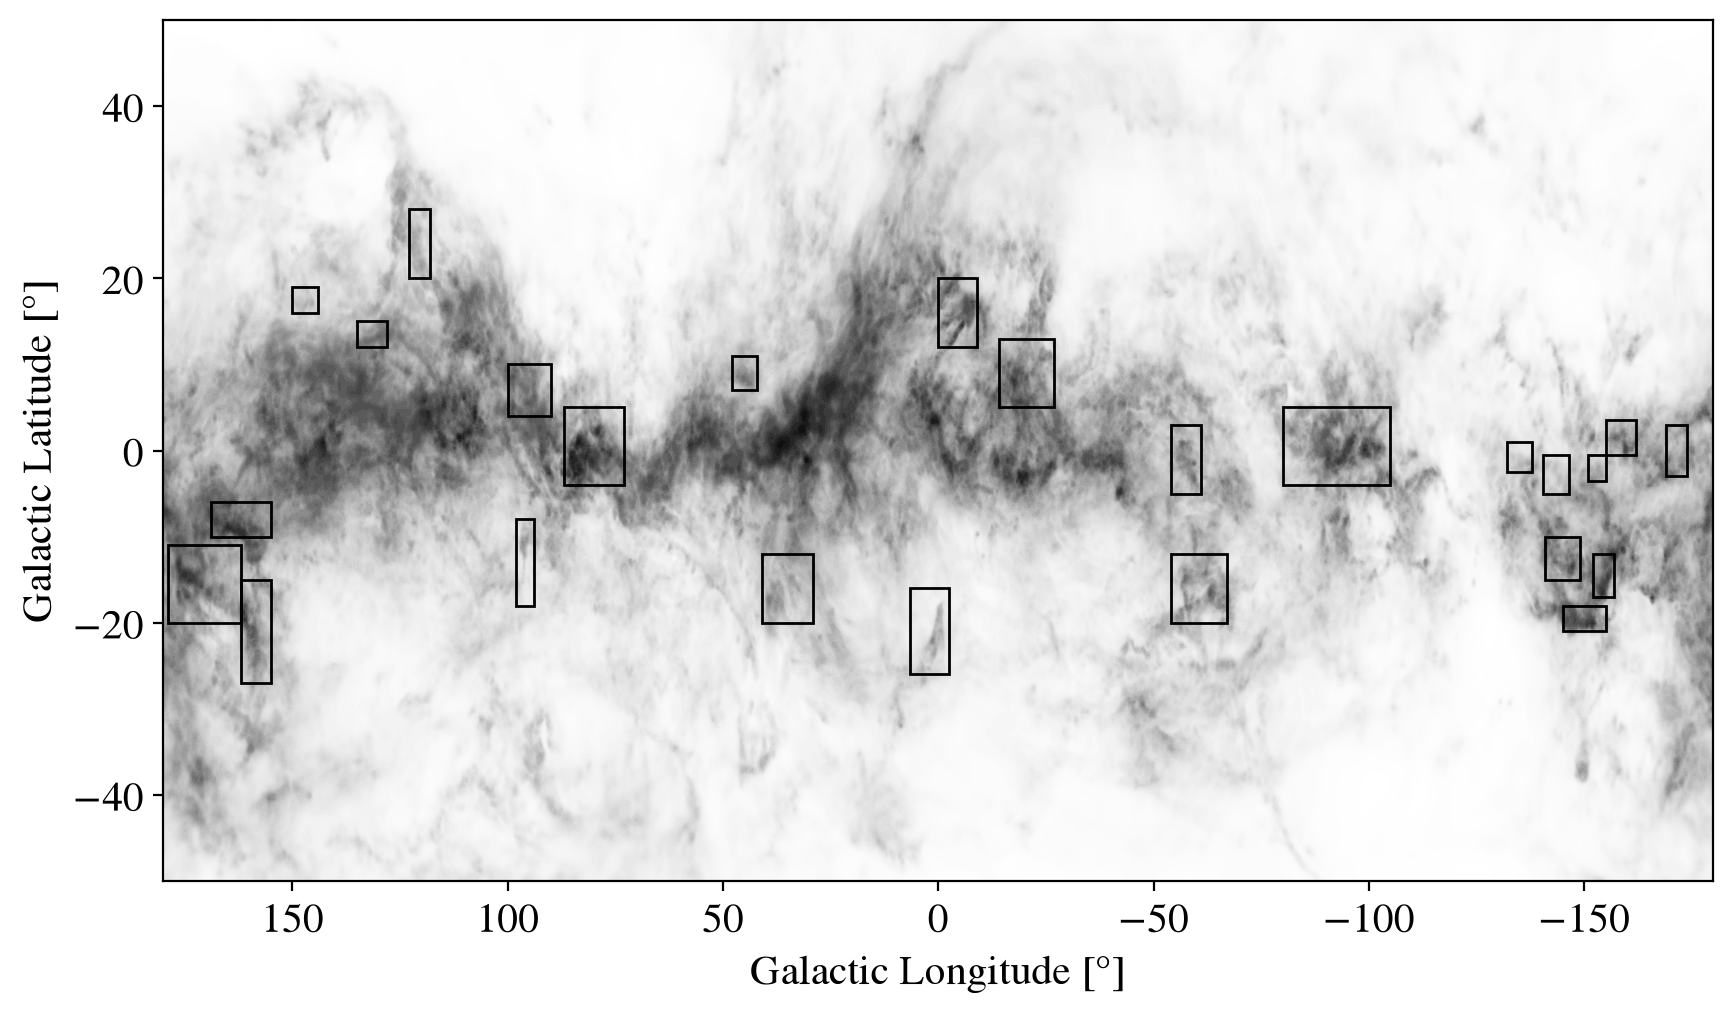
\includegraphics[width=\linewidth]{figures/fig1_catalog.png}
\caption{maps of a molecular cloud (perseus) - orthogonal, with spines overplotted for different distance ranges}
\label{fig1:maps}
\end{figure*}


\textcolor{red}{Figure~\ref{fig:model} shows a labeled illustration of our model. We call the
length of a cloud $L$. In surface density maps of clouds like the Orion Molecular Clouds and the Perseus Molecular Cloud, one can often see that much of the highest
column-density gas is concentrated along a central axis
\citep[e.g.,][]{Lombardi2010, Lombardi2011, Imara2016}, which we will refer to here as the \emph{spine}. The perpendicular distance from the spine to any point
is $r$, and the maximum radius $R_T$ is the distance from the spine to the edge.}

\textcolor{orange}{We define the radial volume density profile of a cloud, $\rho(r)$, as
\begin{align}\label{eq:rho}
\rho = \frac{\rho_0}{\left[1 + \left(\dfrac{r}{r_0}\right)^2\right]^{\alpha}},
\end{align}
where $\rho_0$ is the peak density along the central spine of the cloud, and
$r_0$ is the ``turnover'' radius inside of which the density is roughly constant,
i.e., $\rho \approx \rho_0$. The exponent $\alpha$ describes how quickly the
density falls off beyond $r_0$. Going forward, we refer to the volume density
profile simply as $\rho$ and consider the radial dependence to be implied.}

\textcolor{orange}{The expression for an isothermal cylinder, in which $\alpha = 2$, was derived by
\citet{Stodolkiewicz1963} and \citet{Ostriker1964}:
$\rho_{\mathrm{iso}} = \rho_0[1 + r^2/8r_0^2]^{-2}$. In this instance, the scaling
radius, $r_0$, is equivalent to the Jeans length,
$r_0 = \sqrt{c_s^2 / 4\pi G \rho_0}$, where $c_s$ is the isothermal sound speed.
Clouds with the $\alpha = 2$ profile would have a steeply declining density of
$\rho \propto r^{-4}$ far from the central axis. In observed cylindrical clouds,
however, the density appears to fall off more moderately
\citep[e.g.,][]{Fiege2000, Arzoumanian2011, Toci2015}. In our model, we leave
$\alpha$, $\rho_0$, and $r_0$ as free parameters.
 We note that any variation of
$\rho_0(L)$, which is the density along the spine, is averaged out in the data
(see Equation~\ref{eq:sigmai}), so there is no reason to include it in the model.
Moreover, for simplicity, we assume that $r_0$ does not vary along the symmetry
axis. When we apply Equations~(\ref{eq:rho}) and (\ref{eq:sigmamodel}) to the
data, we are therefore fitting for $\rho_0\cosi$ rather than $\rho_0$ itself,
where $i$ is the angle between the plane of the sky and the cylinder's symmetry
axis.}

\subsection{data\label{sec:obs}}
\textcolor{cyan}{Gaia photometry and parallaxes make it possible to map the line-of-sight extinction due to dust with high angular resolution (down to 0.11 degree). These have various sky and distance coverages (out to x kpc) which make them suitable for () analyses. of the available dust maps, the edenhofer map matches the requirements of the science}

\subsection{Cloud Sample}\label{sec:sample}
\textcolor{cyan}{we start with the set of clouds studied by [zucker 2022], chose the ones with at least one of the sightlines with d < 1.2kpc, average together the measurements to the sightlines ($d_mean, d_std$) and record their spatial extent (lmin, lmax, bmin, bmax) }

\begin{table*}[ht!]
\begin{center}
\caption{Location of molecular clouds and velocities of HI envelopes}
% \begin{tabular}{|l|ll|ll|ll|c|}
\begin{tabular}{|l|cc|cc|c|cc|}
\hline
 Name&  $l_0$&$l_1$&  $b_0$&$b_1$&  $d$&$\overline{v}_\mathrm{HI}$& $\sigma_{v,\mathrm{HI}}$\\ 
\hline
 &  \multicolumn{2}{c|}{$\mathrm{deg}$}&  \multicolumn{2}{c|}{$\mathrm{deg}$}&   $\mathrm{pc}$&\multicolumn{2}{c|}{$\mathrm{km\ s^{-1}}$}\\ 
 \hline
 \hline
 Aquila South&  &&  &&  && \\ 
 California& &&  &&  && \\ 
 Camelopardalis& &&  &&  && \\ 
 Canis Major OB1&&&  &&  && \\ 
 Chamaeleon& &&  &&  && \\ 
 Corona Australis&  && &&  && \\ 
 Crossbones&&& &&  && \\ 
 Gemini OB1&&& &&  && \\ 
 Hercules&  && &&  && \\ 
 Lacerta&  && &&  && \\ 
 Lupus& && &&  && \\ 
 Maddalena& & & & &  && \\
 Monoceros OB1& & & & &  && \\
 Monoceros R2& & & & &  && \\
 Ophiuchus& & & & &  && \\
 Orion A& & & & &  && \\
 Orion B& & & & &  && \\
 $\lambda$-Orionis& & & & &  && \\
 Perseus& & & & &  && \\
 Polaris& & & & &  && \\
 Rosette& & & & &  && \\
 Taurus& & & & &  && \\
 \hline
\end{tabular}
\begin{tablenotes}
    Longitude ($l)$ and latitude ($b$) and distances of the molecular clouds studied here, adapted from \cite{2019ApJ...879..125Z}. The line-center ($\overline{v_\mathrm{HI}}$) and linewidth $\overline{\sigma_\mathrm{HI}}$ are calculated by fitting a plane to the velocity spectrum of the HI envelope associated with each molecular cloud.
\end{tablenotes}

\label{tab:intro}
\end{center}
\end{table*}




%%%%%%%%%%%%%%%%%%%%%%%%%%%%%%%%% OBSERVATIONS %%%%%%%%%%%%%%%%%%%%%%%%%%%%%%%%%%
\section{methods}\label{sec:obs}
\subsection{defining the three-dimensional cloud boundary}


\begin{figure}[ht!]
\centering
\figplaceholder{fig2}
\caption{rho vs r profiles}
\label{fig:maps}
\end{figure}


\begin{figure}[ht!]
\centering
\figplaceholder{fig3}
\caption{Observed radially averaged surface densities (blue circles) as a
function of $\bperp$. Pink shaded areas (pink lines) show the central 68\%
confidence interval (median) for the conditional distribution $\Sigma \mid \bperp$
over a finely sampled range of values for $\bperp$.}
\label{fig:profiles}
\end{figure}

\begin{figure}[ht!]
\centering
\figplaceholder{fig4}
\caption{Results of fitting the explicit cylinder model. Each cloud's median
posterior values of $\rho_0$, $r_0$, and $\alpha$ are plotted, with error bars
showing the central 68\% of the marginal distribution of each parameter. Clouds
with higher central densities $\rho_0$ tend to have more compact centers (lower
$r_0$), but all clouds have $\alpha$ between about 0.5 and 1.}
\label{fig:params}
\end{figure}


\begin{figure}[ht!]
\centering
\figplaceholder{fig5}
\caption{The central density of each cloud relative to its mass and depletion
time. Clouds with higher central densities tend to have lower masses and shorter
depletion times.}
\label{fig:depletion}
\end{figure}

\begin{figure}[ht!]
\centering
\figplaceholder{fig6}
\caption{Inferred density profiles as a function of radial distance. As in
Figure~\ref{fig:profiles}, the conditional posterior distribution at each radius
is represented by a line at the median value for each cloud and a shaded region
showing the central 68\% of the distribution. Here we show the distribution of
$\rho \mid r$ for each cloud. The black dashed line shows
$\rho_{\mathrm{env}} = 10\,(r/\mathrm{pc})^{-1}\,\Msun\,\mathrm{pc}^{-3}$.}
\label{fig:rho}
\end{figure}

\begin{figure}[ht!]
\centering
\figplaceholder{fig7}
\caption{The scaling of cloud mass (left panel) and $\ell_{\parallel,\mathrm{max}}$
and $\bperp{}_{,\mathrm{max}}$ (right panel) with $r_0$. In the right panel, the
$\bperp{}_{,\mathrm{max}}$ have smaller values and the markers are not filled. Both
$\ell_{\parallel,\mathrm{max}}$ and $\bperp{}_{,\mathrm{max}}$ scale with $r_0$ but with a logarithmic slope less than 1.}
\label{fig:scaling}
\end{figure}

\begin{figure}[ht!]
\centering
\figplaceholder{fig8}
\caption{Depletion time as a function of mass, as defined for material within
$A_V > 1$~mag (left) and $A_V > 8$~mag (right). Dashed lines in the right panel
show a factor of $\pm 2$ spread (from the solid line) in dense gas depletion time,
comparable to the extremes of the \citet{Lada2010} result. While we reproduce the
LLA10 result that spread in depletion times becomes smaller when focusing on gas
in high-extinction regions, we do see a trend in both panels that higher-mass
clouds have longer depletion times.}
\label{fig:massdep}
\end{figure}

\textcolor{cyan}{the latitude and longitude bounds of each cloud are used as a guide for where to find the clouds in the edenhofer map. the distances calculated by (zucker? thavisha?) are used as a guide for where to locate the clouds along the line of sight. (x amount of the time, ) the extinction peak at $d_{cloud}$ was the most significant feature along the line of sight, while the remaining () of the time, there were (number or larger) of distinct clouds. is there a correlation between the number of line-of-sight peaks and total integrated mass along the aperture}


\subsection{fitting the spine}
\textcolor{cyan}{to fit the spine we select a subset of the pixels that have $n$ above the 99th percentile threshold of the distribution (Figure showing n-pdf). for (x number of clouds), this n is at () $cm^{-3}$. 
we randomly select a pair of points from among n99, and use them to a define a line as:
\begin{align}
    \textcolor{green}{pt, vector form}
\end{align}
for each of the pixels within the cloud boundary, we calculate the perpendicular distance from this line as 
\begin{align}
    \textcolor{green}{equation from wolfram}
\end{align}
we run scipy minimize + iterate (Nboot times - test a few diff n to make sure results are converged) to get the line that minimizes the sum of distances L1 to the cloud pixels. table 2 lists the pt + vector of each spine}

\textcolor{cyan}{once we have a line defined, we determine the end-points of the spine as follows. Figure 3 shows the parallel profiles (stacked on top of each other, look at if-fig-6). there is (a characteristic length at which the volume density drops - can rparl be scaled by something to line them up ?)


\subsection{radial profiles}

\textcolor{cyan}{
in the process of fitting the spine, we also calculate a corresponding distance cube, which is an array with the same shape as the subcube cut out for the cloud, and where the value of each pixel is its perpendicular distance from the spine, which is calculated as 
\begin{align}
    \textcolor{green}{equation for\ \rperp\ from wolfram}
\end{align}
we calculate the volume radial profile of the clouds by binning the $\rperp$ cube into bins of width = (what was the width) , the volume within each bin is averaged to produce (Figure of radial profiles). 
the conversion from the data units to rho goes as : 
\begin{align}
    \textcolor{green}{n = A_0 \times 2.8 \times A-to-N \times pc to cm^-3}
\end{align}}

\textcolor{cyan}{we derive the model parameters of the cylinder by fitting equation 1 to the radial profiles using scipy curve fit (right now, but do it the way described below).}


%%%%%% fitting with priors and covariance matrix --- include later after incorporating into worflow %%%%%%
% \textcolor{red}{This procedure is repeated $N_{\mathrm{boot}}$ times with slightly different
% choices in the parameters that define the procedure (namely $A_{V,\mathrm{high}}$
% and the adopted distance), and with maps produced by sampling pixels from the
% entire original map with replacement. $A_{V,\mathrm{high}}$ is varied uniformly
% between the 97.5th and 99.5th percentile, and distance is varied by 10\% given the
% observed scatter between the dust-based and VLBI-based distances
% \citep[e.g.,][]{Brunthaler2011, Loinard2013, Reid2014, Reid2016, Zucker2020}. This
% procedure produces $N_{\mathrm{boot}}$ replicates of $\Sigma_i$, allowing us to
% estimate the covariance of the $\Sigma_i$ via the sample covariance:
% \begin{align}\label{eq:cov}
% \hat{S}_{ij} = \frac{1}{N_{\mathrm{boot}}} \sum_{k=1}^{N_{\mathrm{boot}}}
% \left(\Sigma_{i,k} - \bar{\Sigma}_i\right)
% \left(\Sigma_{j,k} - \bar{\Sigma}_j\right),
% \end{align}
% where $\Sigma_{i,k}$ denotes the $k$th replicate of $\Sigma_i$ and
% $\bar{\Sigma}_i$ is the mean value of $\Sigma_i$ across the $N_{\mathrm{boot}}$
% replicates.}

% \textcolor{red}{Given an estimate of $S_{ij}$, we can now reasonably evaluate the likelihood of an
% observed surface density profile $\Sigma_i$ given fixed values of the model
% parameters $\rho_0$, $\alpha$, $r_0$, and $R_T$. To account for additional
% systematic uncertainties, including the deliberately simple nature of the model,
% we also include a parameter $\sigma^2$ that is added to each diagonal component of
% $\hat{S}$. The likelihood is therefore a multivariate normal,}
% \begin{align}\label{eq:likelihood}
% \mathcal{L} &= p\left(\{\Sigma_i\} \mid \rho_0\cosi, \alpha, r_0, R_T,
% \sigma^2\right) \nonumber \\
% &= \frac{1}{\sqrt{(2\pi)^N \det \mathcal{C}}}
% \exp\left(-\tfrac{1}{2} z^{T}\, \mathcal{C}^{-1}\, z\right),
% \end{align}
% where $z$ denotes the displacement vector with components
% \begin{align}\label{eq:z}
% z_i = \Sigma_i - \Sigma_{\mathrm{model}}(\bperp{}_{,i};\, \rho_0\cosi, \alpha,
% r_0, R_T).
% \end{align}
% The covariance matrix has components
% \begin{align}\label{eq:C}
% \mathcal{C}_{ij} = \hat{S}_{ij} + \sigma^2 \delta_{ij},
% \end{align}
% where $\delta_{ij} = 1$ if $i = j$ and 0 otherwise. The $N$ appearing in
% Equation~(\ref{eq:likelihood}) is the number of bins of $\bperp$.

% \textcolor{red}{To fit this model, we need to specify a prior distribution of the model parameters. We choose broad/noninformative priors on the log of each variable independently. These distributions are listed in Table~\ref{tab:priors}. We do impose an upper limit on $\log\sigma^2$ equal to the log of the variance of the $\Sigma_i$, minus an additional $(0.6\,\mathrm{dex})^2$, to remove a branch of the
% posterior distribution in which the physical parameters play no role and all
% variation in the data is attributed to scatter from $\sigma^2$. Samples from the posterior distribution are drawn with the Python package }\texttt{emcee}
% \citep{Goodman2010, ForemanMackey2013}.


\subsection{Cloud Properties}\label{sec:properties}
\textcolor{cyan}{we measure the dust-derived mass of the cloud as 
\begin{align}\label{eq:mass}
\textcolor{green}{M = \sum_j n_{j}\, \partial V}
\end{align}
where the volume element is $\partial V = \Delta l \Delta b \Delta d$,  $\Delta l$ and $\Delta b$ are the (equal)
pixel scales $ = 0.23 degree / pix$. the volume density n at each pixel is calculated from the data units by equation x }

\textcolor{cyan}{the sum is evaluated over the pixels that are within the mask of the cloud }



\begin{table*}\label{tab:m_r_omg_j}
\centering
 % \begin{threeparttable}
 \caption{Physical Properties of Molecular Clouds and their HI envelopes.}

\begin{tabular}{|l|ccc|ccc|c||cccc||cc|c|} 
% \begin{tabular}{|l|ll|ll|ll|ll|ll|ll|} 
% \begin{tabular}{|l|rr|rr|rr|rr|rr|ll|} 

    % \hline
\hline
 Name&  x&  y&z&x hat& y hat& zhat&L& $r_0$& $\rho_0$&$\alpha$&RT&  M&$t_{dep}$& $n_{99}$\\
 \hline
 &  \multicolumn{7}{c||}{spine properties}&\multicolumn{4}{c||}{cylinder properties}& &&\\ 
 \hline
 \hline
 AqS&  &    && & & &&   && && && \\ 
 Cal&  &    && & & &&   && && && \\ 
 Cam&  &    && & & &&   && && && \\ 
 CMO&  &    && & & &&   && && && \\ 
 Chm&  &    && & & &&   && && && \\ 
 CrA& &   && & & &&   && && && \\ 
 Cbn& &   && & & &&   && && && \\ 
 GmO& &   && & & &&   && && && \\ 
 Her& &   && & & &&   && && && \\ 
 Lac& &   && & & &&   && && && \\ 
 Lup& &   && & & &&   && && && \\ 
 Mad& &   && & & &&   && && && \\ 
 MOB& &   && & & &&   && && && \\ 
 MR2& &   && & & &&   && && && \\ 
 Oph& &   && & & &&   && && && \\ 
 OrA& &   && & & &&   && && && \\ 
 OrB& &   && & & &&   && && && \\ 
 $\lambda$Or& &   && & & &&   && && && \\ 
 Per& &   && & & &&   && && && \\ 
 Pol& &   && & & &&   && && && \\ 
 Ros& &   && & & &&   && && && \\ 
 Tau& &   && & & &&   && && && \\ 
\hline
    \end{tabular}
    \begin{tablenotes}
    % \small
    \item Notes: Physical properties calculated from $^{12}\mathrm{CO}$ and 21-cm observations. The properties listed include cloud mass ($M$), radius ($R$), velocity gradient magnitude ($\Omega$) and direction ($\theta$), Pearson coefficient ($\rho$), and specific angular momentum ($j$). The uncertainties in $R$ are calculated from the distance uncertainties reported in \citep{2019ApJ...879..125Z}, and propagated to $j$. The latter is also dependent on the errors of the fit to Equation \ref{eq:v_plane}, which propagate through $\Omega$.
    \end{tablenotes}
    % \end{threeparttable}
\end{table*}

%%%%%%%%%%%%%%%%%%%%%%%%%%%%%%%%%%% RESULTS %%%%%%%%%%%%%%%%%%%%%%%%%%%%%%%%%%%%%
\section{Results}\label{sec:results}
\subsection{spine inclinations and cylindrical profiles}
\textcolor{cyan}{in figure (x) we show the position angles of the spines for the clouds fit in the distance range defined by () - this one should be the large-scale distribution (one face on, one edge-on). in figure we show how the spine inclinations change as a function of distance windows.}

\textcolor{cyan}{Figure \ref{fig:profiles} displays the averaged radial dust volume density
profiles of the clouds in our sample, as well as the cylindrical profile corresponding to the fit parameters calculated in (section 3.3). 
We see that for (x of the cloud) the cylindrical model fits the data well across the full range of $\rperp$.  say more about well behaved clouds.}

\textcolor{cyan}{on the other hand, we find a set of clouds that (what are the different ways the data diverge from the model).}

\textcolor{cyan}{how do the uncertainties (first how do we measure these) correlate with rperp }

\textcolor{cyan}{how do the changes to the inclination affect the profiles, is there anything else that affects them}


\subsection{compare the spine properties and radial volume density profiles between the 2D and 3D cases}
\textcolor{cyan}{link to above, esp through corona australis -- () are cases when the spine identified from 3D has a markedly different on-sky orientation compared to the spine derived from the extinction maps}

\textcolor{cyan}{for each of the eight clouds in imara-forbes, say what is the inclination of the spine they fit vs the one we do. how is the gas distributed along the line-of-sight -- what does this imply about the aspect ratio of the clouds}

\subsection{the relationships between the fit parameters $\rho_0$ $r_0$ $\alpha$ ers bersachew}

\textcolor{cyan}{Figure x shows the relationships between the cylindrical model parameters,
$\rho_0\cosi$, $r_0$, and $\alpha$. what is the relationship between $rho0$ and $r0$
\citet{ImaraForbes} had found that $\rho_0$ is negatively correlated with $r_0$, while the fall-off slope $\alpha$ appears independent of the central density and turnover radius.
other estimates of filamentary density profiles -- \citep[e.g.,][]{Arzoumanian2011, Palmeirim2013, Toci2015, Zucker2018,
Arzoumanian2019}.}

\subsection{the relationships between mass and fit parameters, but also m vs r}
\textcolor{cyan}{we find that }

\subsection{relationship of fit parameters (or sth derived from them) with Star Formation efficiency/ Depletion Time}






\textcolor{red}{Concentrating on $\rho_0\cosi$, which has a strong relationship with $r_0$, we
compare $\rho_0$ to each cloud's mass within its $A_V > 1$ contour and the cloud's
corresponding depletion time, defined as its mass divided by its star formation
rate (Figure~\ref{fig:depletion}). The clouds' SFRs are derived from counts of
their young stellar objects (YSOs) based on infrared data
\citep[e.g.,][]{Hillenbrand1997, Lada2009} and applying the conversion
\begin{align}\label{eq:sfr}
\mathrm{SFR} = N_{\mathrm{YSO}} \cdot 0.25 \times 10^{-6}\, \Msun\,\mathrm{yr}^{-1}
\end{align}
from \citet{Lada2010}. The interested reader may refer to Table~2 of
\citet{Lada2010} for additional references on YSO counts for most clouds, and to
\citet{Gutermuth2011} for MonR2.}

\textcolor{red}{We find that clouds with the highest central volume densities in our sample tend
to have the lowest masses and the shortest depletion times, or equivalently the
highest SFRs relative to their masses. It is to be expected that star formation
might proceed more vigorously in denser gas, given that the freefall time scales
as $\rho^{-1/2}$, but it is less intuitive that higher central volume densities
should correspond to lower masses. We speculate on the ultimate cause of this
correlation in the next section.}


%%%%%%%%%%%%%%%%%%%%%%%%%%%%%%%%% DISCUSSION %%%%%%%%%%%%%%%%%%%%%%%%%%%%%%%%%%%%
\section{Discussion}\label{sec:discussion}
\subsection{comparing different maps / resolutions}
\textcolor{cyan}{in addition to edenhofer, there are a number of dust-derived reconstructions of the three-dimensional structure of the solar neighborhood (cite list). the primary difference between the maps is distance coverage and angular resolution -- with a tradeoff for wider range to lower resolution. we would like to see how robust our results are to resolution and reconstruction method, below we give an overview of how the (spine properties and cylinder fit parameters) calculated above compare to (those derived from the () , (), and () maps).}

\subsection{filamentary flow}
\textcolor{cyan}{plot the position-velocity slices through the spines of (a few well behaved clouds>). is there a converging flow? if so can we calculate a (projected) filament accretion rate? how does this compare to the vazquez=semadeni model
}

\subsection{derive some timescale form the observations - maybe falling inward time and then taht can be compared to depletion time to say something}
\textcolor{red}{The clouds' central volume densities
$\rho_0\cosi$ seem to be closely tied to their scale radii $r_0$, their masses
$M_{A_V > 1}$, and their depletion times $M_{A_V > 1}/\mathrm{SFR}$, but with
little correspondence to their outer power-law slopes $-2\alpha$ or their
truncation radii $R_T$. To delve into these potential relationships, we have found
it helpful to plot the inferred density profiles as a function of radial distance
from the spine in Figure~\ref{fig:rho}.}

\textcolor{red}{While there is still a fair amount of variety between the clouds, some of which may
come from the unknown inclination $i$, we see that, roughly speaking, the clouds'
density profiles fit within an envelope of
$\rho_{\mathrm{env}} \approx 10\,(r/\mathrm{pc})^{-1}\,\Msun\,\mathrm{pc}^{-3}$,
with each cloud having a different radius and density at which it turns over and
flattens toward $r \to 0$. In this sense, the relationship between $r_0$ and
$\rho_0\cosi$ becomes clear: the higher the central density, the smaller the
turnover radius must be in order to remain within the $\rho_0\cosi \lesssim 1/r$
envelope.}



\textcolor{red}{The interpretation of the clouds' density profiles as lying within this envelope
also helps explain the clouds' masses, and in particular the somewhat surprising
fact that clouds with higher central densities have lower total masses. As long as
$\rho(r)$ is less steep than $1/r$ near the cloud center, the exact density profile
in the central pc will not have a large effect on the cloud's mass. Instead, the
clouds' masses will be dominated by the large-radius behavior, for which we can use
the $1/r$ envelope, obtaining
\begin{align}\label{eq:massenv}
M \sim \int 2\pi\, r\, \rho_{\mathrm{env}}\, dr
\approx 70\, \Msun \left(\frac{\ell_{\parallel,\mathrm{max}}}{\mathrm{pc}}\right)
\left(\frac{\bperp{}_{,\mathrm{max}}}{\mathrm{pc}}\right).
\end{align}
This is equivalent to stating that within the boundary of the cloud, the average
surface density is $\sim$70~$\Msun\,\mathrm{pc}^{-2}$, similar to Larson's classic
result \citep{Larson1981} and more recent results on molecular filaments
\citep{Zhang2019}.}

\textcolor{red}{The star formation rate, meanwhile, is expected to obey some relationship with the
volume density of the gas \citep{Schmidt1959, Kennicutt2012}. For volume
densities, the density of the star formation rate is commonly expressed as
\begin{align}\label{eq:rhosfr}
\rho_{\mathrm{SFR}} = \frac{\epsilon_{\mathrm{ff}}\, \rho}{t_{\mathrm{ff}}},
\end{align}
where $\epsilon_{\mathrm{ff}}$ is an efficiency factor of order 1\%
\citep[e.g.,][]{Krumholz2007, Krumholz2012}, and the freefall time
$t_{\mathrm{ff}} = \sqrt{3\pi/32 G \rho}$. Interestingly, integrating
Equation~(\ref{eq:rhosfr}) over the volume of the model cylinders does not
reproduce the observed SFRs as measured by YSO counts, except for California and
Rosette. In most other clouds, Equation~(\ref{eq:rhosfr}) applied to the smooth
model falls short of the actual SFR by about a factor of 10, because our smoothed
distribution averages out high-density peaks.}

\textcolor{red}{While the inferred large-scale density distribution of the cloud cannot be used to
infer the SFR directly by integration of Equation~(\ref{eq:rhosfr}), there is still
a trend between the depletion time and the parameters of the large-scale cloud
model. Very roughly, $t_{\mathrm{dep}} \propto (\rho_0\cosi)^{-1}$.}

\textcolor{red}{\citet{Lada2010}, hereafter LLA10, showed using the same dust extinction data and
a similar sample of local molecular clouds that depletion time has no discernible
trend with cloud mass, defined as mass within the $A_V = 1$ contour, and that the
spread in depletion times becomes much smaller when using the mass within a contour
of $A_V \gtrsim 8$. In Figure~\ref{fig:massdep}, we show the trends between mass and
depletion time for both $A_V > 1$ and $A_V > 8$. Where LLA10 found no trend with
total mass, we find that higher-mass clouds have longer depletion times, regardless
of whether we look at total mass or dense mass. We do recover the main result that
the scatter in depletion times is substantially reduced when looking at the dense
mass, though not quite as much as in LLA10.}

\textcolor{red}{We can attribute \textcolor{cyan}{the differences from LLA10} to four factors: first, we have used
updated distances to the clouds based on Gaia distances \citep{Zucker2020};
second, we have used a somewhat different selection of clouds; third, we have used
slightly different definitions of the clouds and their masses; and fourth, our
method produces confidence intervals for the cloud masses, which changes the
assessment of which trends are plausible versus implausible.}

\textcolor{red}{While our results provide an interesting new perspective on well-studied local molecular clouds, they also have broader implications. Models in a variety of contexts depend explicitly or implicitly on breaking the star formation rate in a
patch of the interstellar medium, a whole galaxy, or even across galaxies, into a population of molecular clouds \citep{Chevance2020, Tacchella2020}. This variability has been invoked to explain the discovery by JWST of galaxies at $z \sim 6$ that have, at least momentarily, stopped forming stars
\citep{Dome2023}. Extragalactic surveys with large sample sizes are able to constrain the cloud scaling relations that enter into these models
\citep[e.g.,][]{Hughes2013, Faesi2018, Rosolowsky2021}. Just as the global star formation rate can be broken into its contributions from individual clouds, the line luminosities from star-forming regions at high redshift are summed from individual clouds \citep{Krumholz2014, Narayanan2014, Narayanan2017}, \textcolor{cyan}{and} changes in the underlying assumptions about the typical morphology of clouds may alter the inference of the galaxy property distribution \citep{Zhang2023} from forthcoming emission line intensity mapping surveys \citep[e.g.,][]{Pullen2023}.}

%%%%%%%%%%%%%%%%%%%%%%%%%%%%%%%%%%% SUMMARY %%%%%%%%%%%%%%%%%%%%%%%%%%%%%%%%%%%%%
\section{Summary}\label{sec:summary}
We \textcolor{cyan}{test the Imara-Forbes cylindrical model of global molecular cloud morphology using dust-extinction derived three-dimensional reconstructions of the solar Neighborhood. [we test a set of 3d maps ?] and find that the spines fitted for each cloud are (different not) between them. (number) of the clouds have global 3d structure that is well fit by the imara forbes model, while () have radial profiles that (). how do the 3d values compare to 2d from extinction. we derive relationships between the fit parameters and find that }

\begin{enumerate}
 \textcolor{cyan}{\item  we find a () relationship between the central volume density $\rho_0$ and the turnover radius $r_0$, (imara forbes find anticorrelation implying that clouds with higher $\rho_0$ are more compact).}
 \textcolor{red}{\item Somewhat surprisingly, clouds with higher central densities have lower total
      masses. This is because the density profile in the central pc does not have
      a large effect on a cloud's mass, as long as $\rho(r)$ is less steep than
      $1/r$ near the cloud center. Clouds' masses will be dominated by the
      large-radius behavior, described by the $1/r$ envelope.
\item Higher-mass clouds have longer depletion times, regardless of whether we
      consider their total mass or dense mass.
\item While the overall dense gas fraction of molecular clouds helps to explain
      some of the variation in the depletion time, our results show that the global
      cylindrical structure of clouds---reflected, for instance, in the central
      volume density---plays a key role in determining $t_{\mathrm{dep}}$.
\end{enumerate}}

\begin{acknowledgements}
acknowledgements
\end{acknowledgements}

\software{emcee \citep{ForemanMackey2013},
          corner \citep{ForemanMackey2016}}
          \textcolor{cyan}{astropy scipy numpy pandas }

\bibliography{references}
\bibliographystyle{aasjournalv7}

%%%%%%%%%%%%%%%%%%%%%%%%%%%%%%%%%%% APPENDIX %%%%%%%%%%%%%%%%%%%%%%%%%%%%%%%%%%%%
\appendix
\counterwithin{figure}{section}

\section{model parameters depend on ()}\label{sec:appendix}

\textcolor{cyan}{once i get to where i'm fitting the cloud $b_perp$ (and $b_parl?$) profiles, look into making corner plots and show one here. what are the variables that we trust, what are the variables that hsow degeneracies and is there anything that would break these degeneracies. what does this mean in terms of the conclusions that we draw.}


\begin{figure}[ht!]
\centering
\figplaceholder{fig9}
\caption{A corner plot for our model fit to the Orion B molecular cloud. The
histograms on the diagonal show the 1D marginal posterior distributions of the five
parameters in the model, while the off-diagonal plots show each 2D marginal
posterior distribution, representing the distribution through a combination of
contours and individual points in less sparsely populated areas.}
\label{fig:corner}
\end{figure}


\end{document}
